\label{The Netstat Command}
\chapter{The Netstat Command}

To investigate the netstat command, you can either use any Linux machine, or you can create a Kathara node.

Summary: netstat command provides information about the network connections, the ports that are in use, and the processes using them. 
The -a (all) option makes netstat show all the connected and waiting sockets. As shown below:
\textsl{ netstat -a}

\begin{figure}[H]
\Centering
  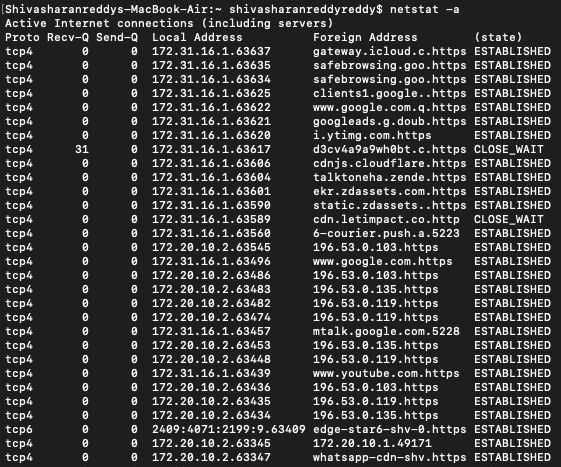
\includegraphics[width=0.6\textwidth]{Images/Image1-1-Netstat.jpg}
  \caption{netstat Command}
  \label{fig:1.1}
\end{figure}

\section{Display the information on the TCP and UDP ports that are currently in use.}
\textsl{ netstat -aut}
\begin{figure}[H]
\centering
  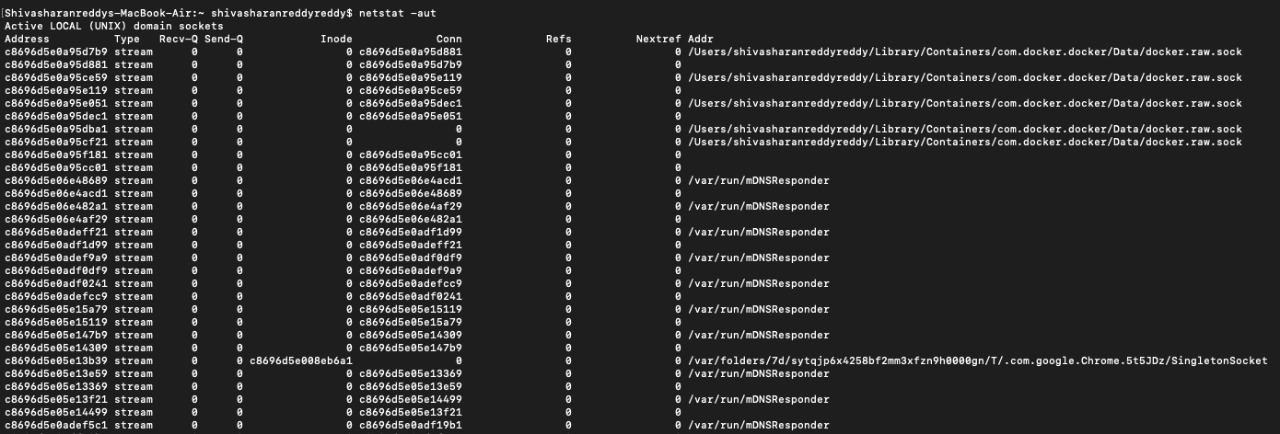
\includegraphics[width=0.6\textwidth]{Images/Image1-2-netstatTCPUDP.jpg}
  \caption{netstat Command showing TCP and IP ports in use}
  \label{fig:1.2}
\end{figure}
\section {Display the statistics of the various networking protocols}
\textsl{ netstat -s} 
\begin{figure}[H]
\centering
  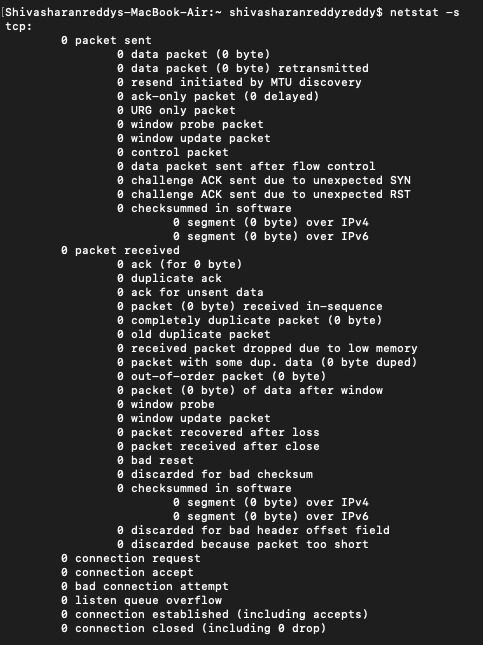
\includegraphics[width=.6\textwidth]{Images/Image1-3-NetstatStatistics.jpg}
  \caption{netstat Command, Showing only TCP ports}
  \label{fig:1.3}
\end{figure}
\section {Suppose you want to write a small application that needs the process id (PID) of
a given application. In order to achieve this, use a command of your choice, e.g.
grep, sed or awk, to filter the output of netstat. Your application should only deliver
the port number of a particular application (e.g. inetd or sshd), identified by the
PID, as parameter.}
Command in Linux: 
\textsl{ netstat -anp |grep "sshd" } 
\newline
* As there is not enough network activities working with Kathara, the equivalent option windows (findstr) has been run.
\newline 
The command is:
\textsl{ netstat -a -n -p |findstr 8452 }
\newline 8452 for example, is the PID for windows host process.
Here is the result: 
\begin{figure}[H]
\centering
  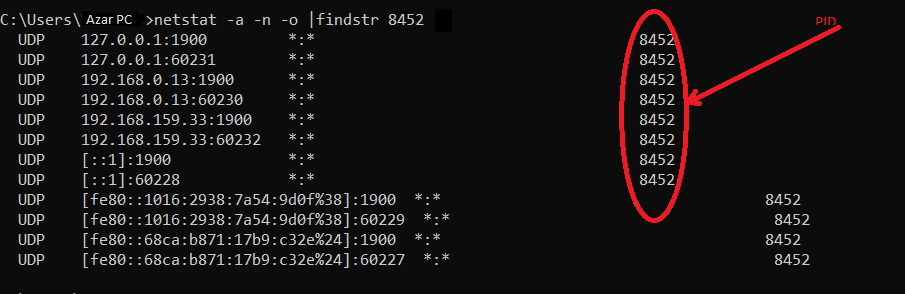
\includegraphics[width=.6\textwidth]{Images/Image1-4-Netstatgrep.png}
  \caption{grep command to filter output of netstat}
  \label{fig:1.4}
\end{figure}



